\chapter{\label{chap:ngram}N-grams}
%TODO: better chapter title

In this chapter we will study \emph{n-gram language models},
which we will call simply \emph{language models},
and sometimes we will even disregard
the distinction between the model and the sequence,
and call them \emph{n-grams}, following the common practice in the field.
The models we will discuss here are very simple,
yet very effective in many practical natural language applications.
The main idea is given a sequence of words,
we want to assign a probability to the sequence,
based on a short context of each word in the sequence.
These probabilities allow us to select the more likely sequence,
e.g., sentence or utterance, among other alternatives.
Before going into details,
we will motivate their use with a few examples.

\section{Example applications of n-gram language models}
Assume that you are developing a spell checker.
With a good enough lexicon,
it is not difficult to catch the spellling error in this sentence.
For morphologically complex languages,
you may need help from some morphological rules
to define the valid words in the language rather than listing them,
but once you have such a system that defines the valid words,
it is easy to spot spelling errors within words.
But, how about the spelling error in (\getref{spell-wit}) below?

\ex<spell-wit>
  I don't like pizza \emph{wit} spinach.
\xe

If we have a lexicon with word frequencies,
one way to to solve this problem would
be pay attention to \emph{confusables} of high-frequency words like \emph{with}.
Here, we may be able to rely on the fact that $P(\text{with}) > P(\text{wit})$.
This still does not solve the problem if the spelling correction is to be made non-interactively.
Choosing the high-frequency confusable does not guarantee correctness:
in another spelling error we may have \emph{with} instead of \emph{wit}.
Furthermore,
consider the news headline in (\getref{spell-lose}).

\ex<spell-lose>
  Zoo animals on the \emph{lose}
\xe

The word frequency (or probability) does not help here,
if you compare the frequencies of the words in Google Books Ngram Viewer,%
\footnote{\url{https://books.google.com/ngrams/graph?content=lose\%2C+loose}}
you will see that \emph{lose} has been more common
than the correct form in this example, \emph{loose},
in the most part of the history of written English.
Even though $P(\text{loose}) < P(\text{lose})$,
any competent speaker would agree that the relations between
the probabilities of complete sequences should be 
$P(\text{Zoo animals on the \emph{loose}}) > P(\text{Zoo animals on the \emph{lose}})$.
As a result,
we want our language model to assign probabilities to these sequences accordingly.

Those who took a parsing course before may (rightfully)
suggests parsing as a solution.
Indeed,
a structure-sensitive language model (e.g., a parser) would be helpful.
However,
parsing is a rather complex task.%
\footnote{Parsing is the most popular sport in computational linguistics.
  Like many sports, it is fun, but challenging -
  it is computationally `heavy' and requires resources (treebanks)
  that are expensive to build.
  Although we (computational linguists) have been enthusiastic about our sport,
  in most practical applications,
  simpler solutions (like the ones we will discuss in this chapter)
  often work better -
  or well enough that complexity of parsing is not warranted.
}
The n-gram models that we will discuss in this chapter are much simpler,
yet effective enough that they are the dominant method for language modeling
in many of the practical applications.
The basic idea is to estimate the probability of a sequence,
such as a sentence,
from its parts (the words),
and to estimate the probabilities of the words,
pay attention to the context of the word.

The spelling correction example above is not the only application for n-grams.
There are many applications of the n-gram language models.
For example,
in automatic speech recognition (ASR),
the speech signal often gives rise to multiple possible word sequences.
A well-known example is presented in Figure~\ref{fig:wreck},
where all possible word sequences that are compatible
with the \emph{phone}s identified from the speech signal are represented in a lattice.
Each path that spans all the phones is a candidate utterance,
among which we can trace \emph{wreck a nice beach},
as well as the expected \emph{recognize speech}.
Even if the former may be more likely based on the analysis of the signal,
an n-gram model scoring the sequences is likely to select the latter,
at least if the n-gram model was trained on language samples of NLP domain.
\begin{marginfigure}
  \tikzsetnextfilename{wreck-a-nice-beach}
  \begin{tikzpicture}[every node/.style={anchor=south,inner ysep=0.1em,font=\tiny},
                      x=5mm
    ]
    \foreach \x/\l in {0/r,1/e,2/k,3/@,4/n,5/ai,6/s,7/b,8/ii,9/ch}{%
      \draw ($ (\x, 0) + (0.5, 0) $)  node[anchor=base,font=\scriptsize] {\l};
    }

    \pgfsetcornersarced{\pgfpoint{2mm}{2mm}}
    \def\height{0.3}

    \pgfmathsetmacro{\y}{1*\height}
    \draw (3,0) -- (3,\y) -- node {her} (4,\y) -- (4,0);
    \draw (4,0) -- (4,\y) -- node {and} (5,\y) -- (5,0);
    \draw (5,0) -- (5,\y) -- node {I} (6,\y) -- (6,0);
    \draw (6,0) -- (6,\y) -- node {s} (7,\y) -- (7,0);
    \draw (7,0) -- (7,\y) -- node {be} (9,\y) -- (9,0);

    \pgfmathsetmacro{\y}{2*\height}
    \draw (3,0) -- (3,\y) -- node {a} (4,\y) -- (4,0);
    \draw (4,0) -- (4,\y) -- node {aren't} (5,\y) -- (5,0);
    \draw (5,0) -- (5,\y) -- node {ice} (6,\y) -- (6,0);
    \draw (7,0) -- (7,\y) -- node {bee} (9,\y) -- (9,0);

    \pgfmathsetmacro{\y}{3*\height}
    \draw (4,0) -- (4,\y) -- node {an} (5,\y) -- (5,0);
    \draw (5,0) -- (5,\y) -- node {eye} (6,\y) -- (6,0);
    \draw (7,0) -- (7,\y) -- node {beach} (10,\y) -- (10,0);

    \pgfmathsetmacro{\y}{4*\height}
    \draw (4,0) -- (4,\y) -- node {not} (5,\y) -- (5,0);

    \pgfmathsetmacro{\y}{5*\height}
    \draw (4,0) -- (4,\y) -- node {nice} (7,\y) -- (7,0);

    \pgfmathsetmacro{\y}{6*\height}
    \draw (3,0) -- (3,\y) -- node {an} (5,\y) -- (5,0);

    \pgfmathsetmacro{\y}{7*\height}
    \draw (3,0) -- (3,\y) -- node {aren't} (5,\y) -- (5,0);
    \draw (6,0) -- (6,\y) -- node {speech} (10,\y) -- (10,0);

    \pgfmathsetmacro{\y}{8*\height}
    \draw (3,0) -- (3,\y) -- node {in} (5,\y) -- (5,0);
    \draw (5,0) -- (5,\y) -- node {ice} (7,\y) -- (7,0);
    \draw (7,0) -- (7,\y) -- node {speech} (10,\y) -- (10,0);

    \pgfmathsetmacro{\y}{9*\height}
    \draw (0,0) -- (0,\y) -- node {wreck} (3,\y) -- (3,0);
    \draw (3,0) -- (3,\y) -- node {on} (5,\y) -- (5,0);

    \pgfmathsetmacro{\y}{10*\height}
    \draw (0,0) -- (0,\y) -- node {reckon} (5,\y) -- (5,0);

    \pgfmathsetmacro{\y}{11*\height}
    \draw (0,0) -- (0,\y) -- node {recognize} (7,\y) -- (7,0);
  \end{tikzpicture}
  \caption{\label{fig:wreck}%
    An automatic speech recognizer's attempt to recognize
    the phrase \xmpl{recognize speech}.
    Example re-produced from \parencite{shillcock1995}.
  }
\end{marginfigure}

A very similar use case also arise in machine translation (MT).
The classical statistical MT systems produce
many alignments between the source and target languages,
and a language model of the target language is used
for picking the most fluent option.
For example the German phrase \xmpl{Er tanzt gerne} can be translated as
`He dances with-pleasure' or `He likes to dance'.
Although both are acceptable translations,
a language model of English is expected to pick the more fluent (second) option.

% TODO:
% All three examples above are typically modeled
% using the noisy channel model discussed in Chapter~\ref{chap:information-theory}
% 
% \begin{marginfigure}
%   \tikzsetnextfilename{noisy-channel}
%   \begin{tikzpicture}
%     \node (in) {a};
%     \node[draw,thick,right=3mm of in, minimum height=4ex] (enc) {encoder};
%     \node[draw,thick,right=15mm of enc, minimum height=4ex] (dec) {decoder};
%     \node[right=3mm of dec] (out) {a};
%     \draw[thick,->] (in) -- (enc);
%     \draw[thick,->] (dec) -- (out);
%     \draw[thick,decorate, decoration={snake,post length=1mm},->]
%       (enc) -- (dec)
%       node[midway, above,yshift=2mm,font=\small,text width=1cm,align=center]
%         {noisy\\channel};
%   \end{tikzpicture}
%   \caption{\label{fig:noisy-channel}%
%   }
% \end{marginfigure}
% 

In the examples above,
we were interested in assigning probabilities (or scores) to a sequence of words.
Another application of the language models is in predicting the next word.
This is commonly used in text boxes in web applications,
such as query input of a search engine.
Note that although most of our examples were about words,
we may need to score sequences of other linguistic units,
such as letters or phonemes.
An example of predictive text based on letters is found
in mobile phone virtual keyboards,
which helps phone users typing short messages quickly.
Figure~\ref{fig:google-predictive-text} shows screenshots
from a web application with predictive text
using both word- and character-level models.
\begin{marginfigure}
  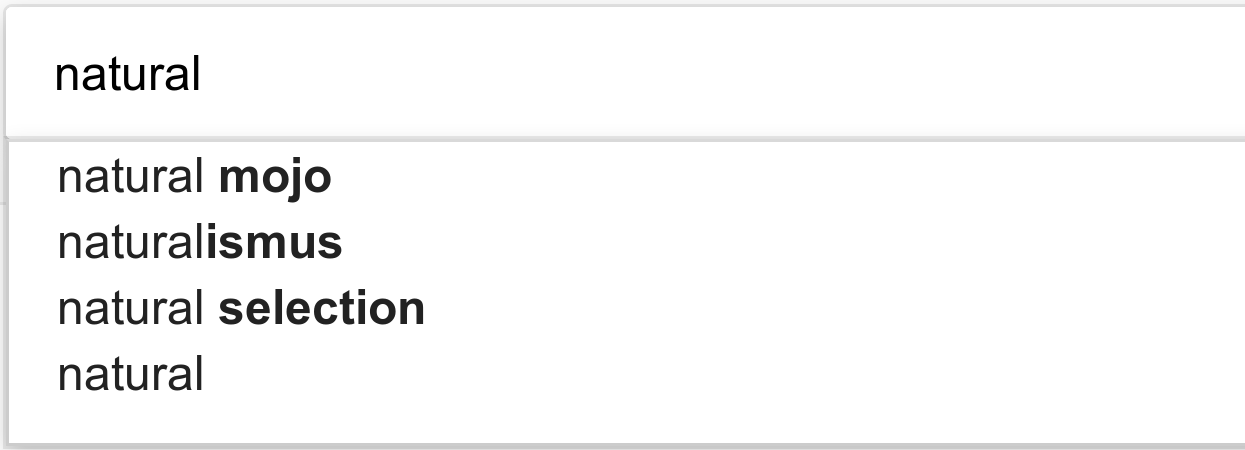
\includegraphics[width=\textwidth]{figures/google-predictive-text-1.png}\\
  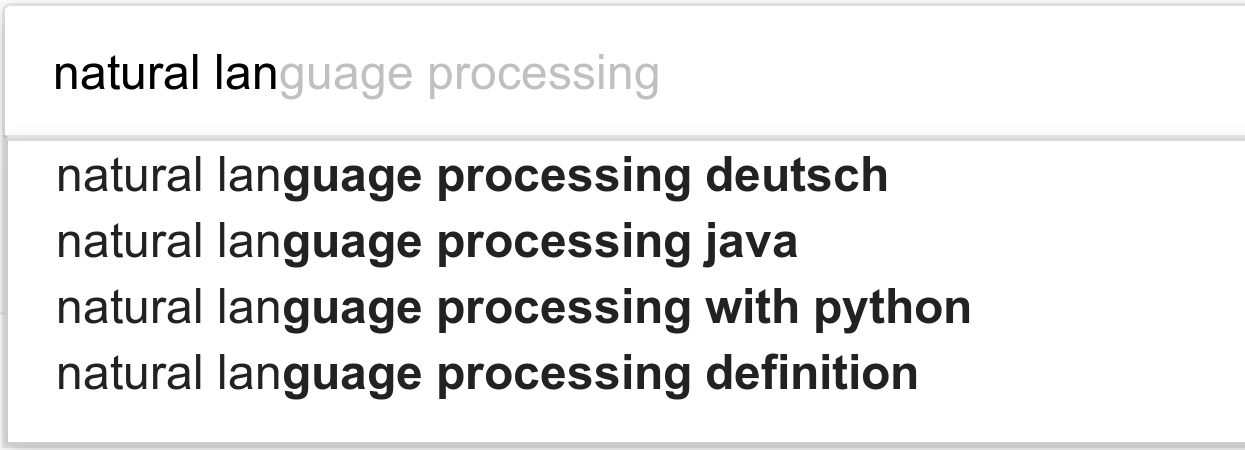
\includegraphics[width=\textwidth]{figures/google-predictive-text-2.png}
  \caption{\label{fig:google-predictive-text}%
    Predictive text on a web search engine in two steps (from google.com).
    Although we do not know exact nature of the language models Google uses,
    n-gram language models we discuss here are definitely a good guess.
    Note that there are two different n-grams models are in action here.
    One predicting the next words based on the previous words,
    and another one predicting the (remaining) characters
    in the word being typed,
    based on previous characters.
  }
\end{marginfigure}

The examples above should be enough for motivating
the n-gram language models,
although there are many more applications of this simple method.
In this chapter we will define them,
discuss important issues and some of the important aspects of estimation,
and mention some of the extensions or advanced usages of n-grams.

\section{Estimating probabilities of n-grams}

N-grams are simply a fixed length sequences of words
(or other units, such as letters).
The length of an n-gram is determined by the `n' in the name.
N-grams of length one, \emph{unigrams}, are simply the words without context.
N-grams of length two and three also have special names,
\emph{bigrams} and \emph{trigrams},
and they are formed by sequences of two and three words respectively.
Larger n-grams are are generally called four-grams, five-grams and so on.

We will use the first articles of the declaration of human rights
for demonstrating what constitutes an n-gram.

%\begin{lstlisting}[language=,basicstyle=\small,breaklines=true]
\begin{tcolorbox}
All human beings are born free and equal in dignity and rights .
They are endowed with reason and conscience and should act towards one another in a spirit of brotherhood .
\end{tcolorbox}
%\end{lstlisting}


\section{Estimating probabilities word sequences}

\section{What is wrong with MLE of n-grams}

\section{Smoothing and back-off}

\subsection{Add-one smoothing}

\section{Extensions}

\section{Rewritten material}

In many natural language applications,
we want to know how likely a particular sequence of units
(words, phonemes, characters, \ldots) is.
For example,
for both practical and theoretical reasons,
we want our computational methods to indicate that 
the sentence (\getfullref{ngram-chomsky.a}) is a likely sentence in English.
The sentence (\getfullref{ngram-chomsky.b}),
on the other hand,
is unlikely
(at least if we discount its usage as a grammatical but nonsense sentence).%
\footnote{%
  All examples except (\getfullref{ngram-chomsky.a}) are from
  \textcite{chomsky1957}.
}
The sentence (\getfullref{ngram-chomsky.c}) is even more unlikely,
it is ungrammatical.
It would probably have never been observed in real language use
if it was not used by Chomsky as an ungrammatical sentence example.
Unlike (\getfullref{ngram-chomsky.e}),
the sentence (\getfullref{ngram-chomsky.d}) is also a common example of
an ungrammatical sentence,
but most native speakers would not have much difficulty to assign
an interpretation (most likely `the child seems to be sleeping') to it
\parencite[p210]{chater2015}.

\pex<ngram-chomsky>
%TODO: better example (the first one)?
  \a<a> Tired little children sleep quietly.
  \a<b> Colorless green ideas sleep furiously.
  \a<c>\ljudge{*} Furiously sleep ideas green colorless.
  \a<d>\ljudge{*} The child seems sleeping.
  \a<e> The book seems interesting.
\xe
Clearly,
we do not want to treat the sentences in (\getref{ngram-chomsky}) the same.
Word ngrams,
or \emph{language models} have been one of the simple but successful methods
for determining which sequences of words are more likely in a language.%
Although their success on capturing
many linguistic dependencies are questionable,
ngram language models have been very useful in practical NLP applications,
ranging from speech recognition to machine translation.
For example,
simple ngram language models like the ones we will discuss can be useful in
\begin{itemize}
  \item spelling correction,
    although all words in \emph{I ate pizza wit spinach}
    are correct words, a language model could easily signal that 
    \emph{I ate pizza wit\textbf{h} spinach} is a more likely sequence.
  \item machine translation
  \item speech recognition
\end{itemize}

\section*{Where to go from here}

\textcite{chen1998} includes a tutorial on most of the smoothing techniques,
followed by an empirical comparison of them.

\section*{Exercises}

\begin{question}
  Which one of the following is a more probably sentence English according to a typical unigram model?
  \begin{itemize}
    \item Furiously sleep ideas green colorless.
    \item Colorless green ideas sleep furiously.
    \item Tired little children sleep quietly. 
    \item the the the the.
  \end{itemize}
\end{question}

\begin{question}
  How do you fix the problem in the previous question?
\end{question}

\begin{question}
  What is perplexity, what does it tell us?
\end{question}

\begin{question}
  Write a python program that calculates bi-gram frequencies for a given corpus.
\end{question}

\begin{question}
  Show that the formula below (to be used earlier),
  corresponds to cross entropy between the distribution defined
  by the n-gram model
  and the MLE estimate of the distribution of words
  in the test corpus.

  \[
    H_{P}(T) = - \frac{1}{\lvert{}T\rvert{}}log_{2}P(T)
  \]
  where P is the probability assigned to a word (sequence)
  by an n-gram model trained on the training corpus,
  T is the test set ($\lvert{}T\rvert{}$ is its size).

\end{question}
